\documentclass{beamer}
\usepackage[latin1]{inputenc}
\usefonttheme[onlylarge]{structurebold}
\setbeamerfont*{frametitle}{size=\normalsize,series=\bfseries}
\setbeamertemplate{navigation symbols}{}
\usetheme{Goettingen}
\defbeamertemplate{itemize item}{checkbox}{\Square}
\defbeamertemplate{itemize item}{checked}{\Square\llap\CheckmarkBold}

\title[Lab Meeting II]{Lab Meeting II}
\author{Carles Boix}
\begin{document}

\begin{frame}
    \begin{center}
        {\large \textsc{Last Week (11/11):}}
    \end{center}
    \begin{figure}[ht!]
        \centering
        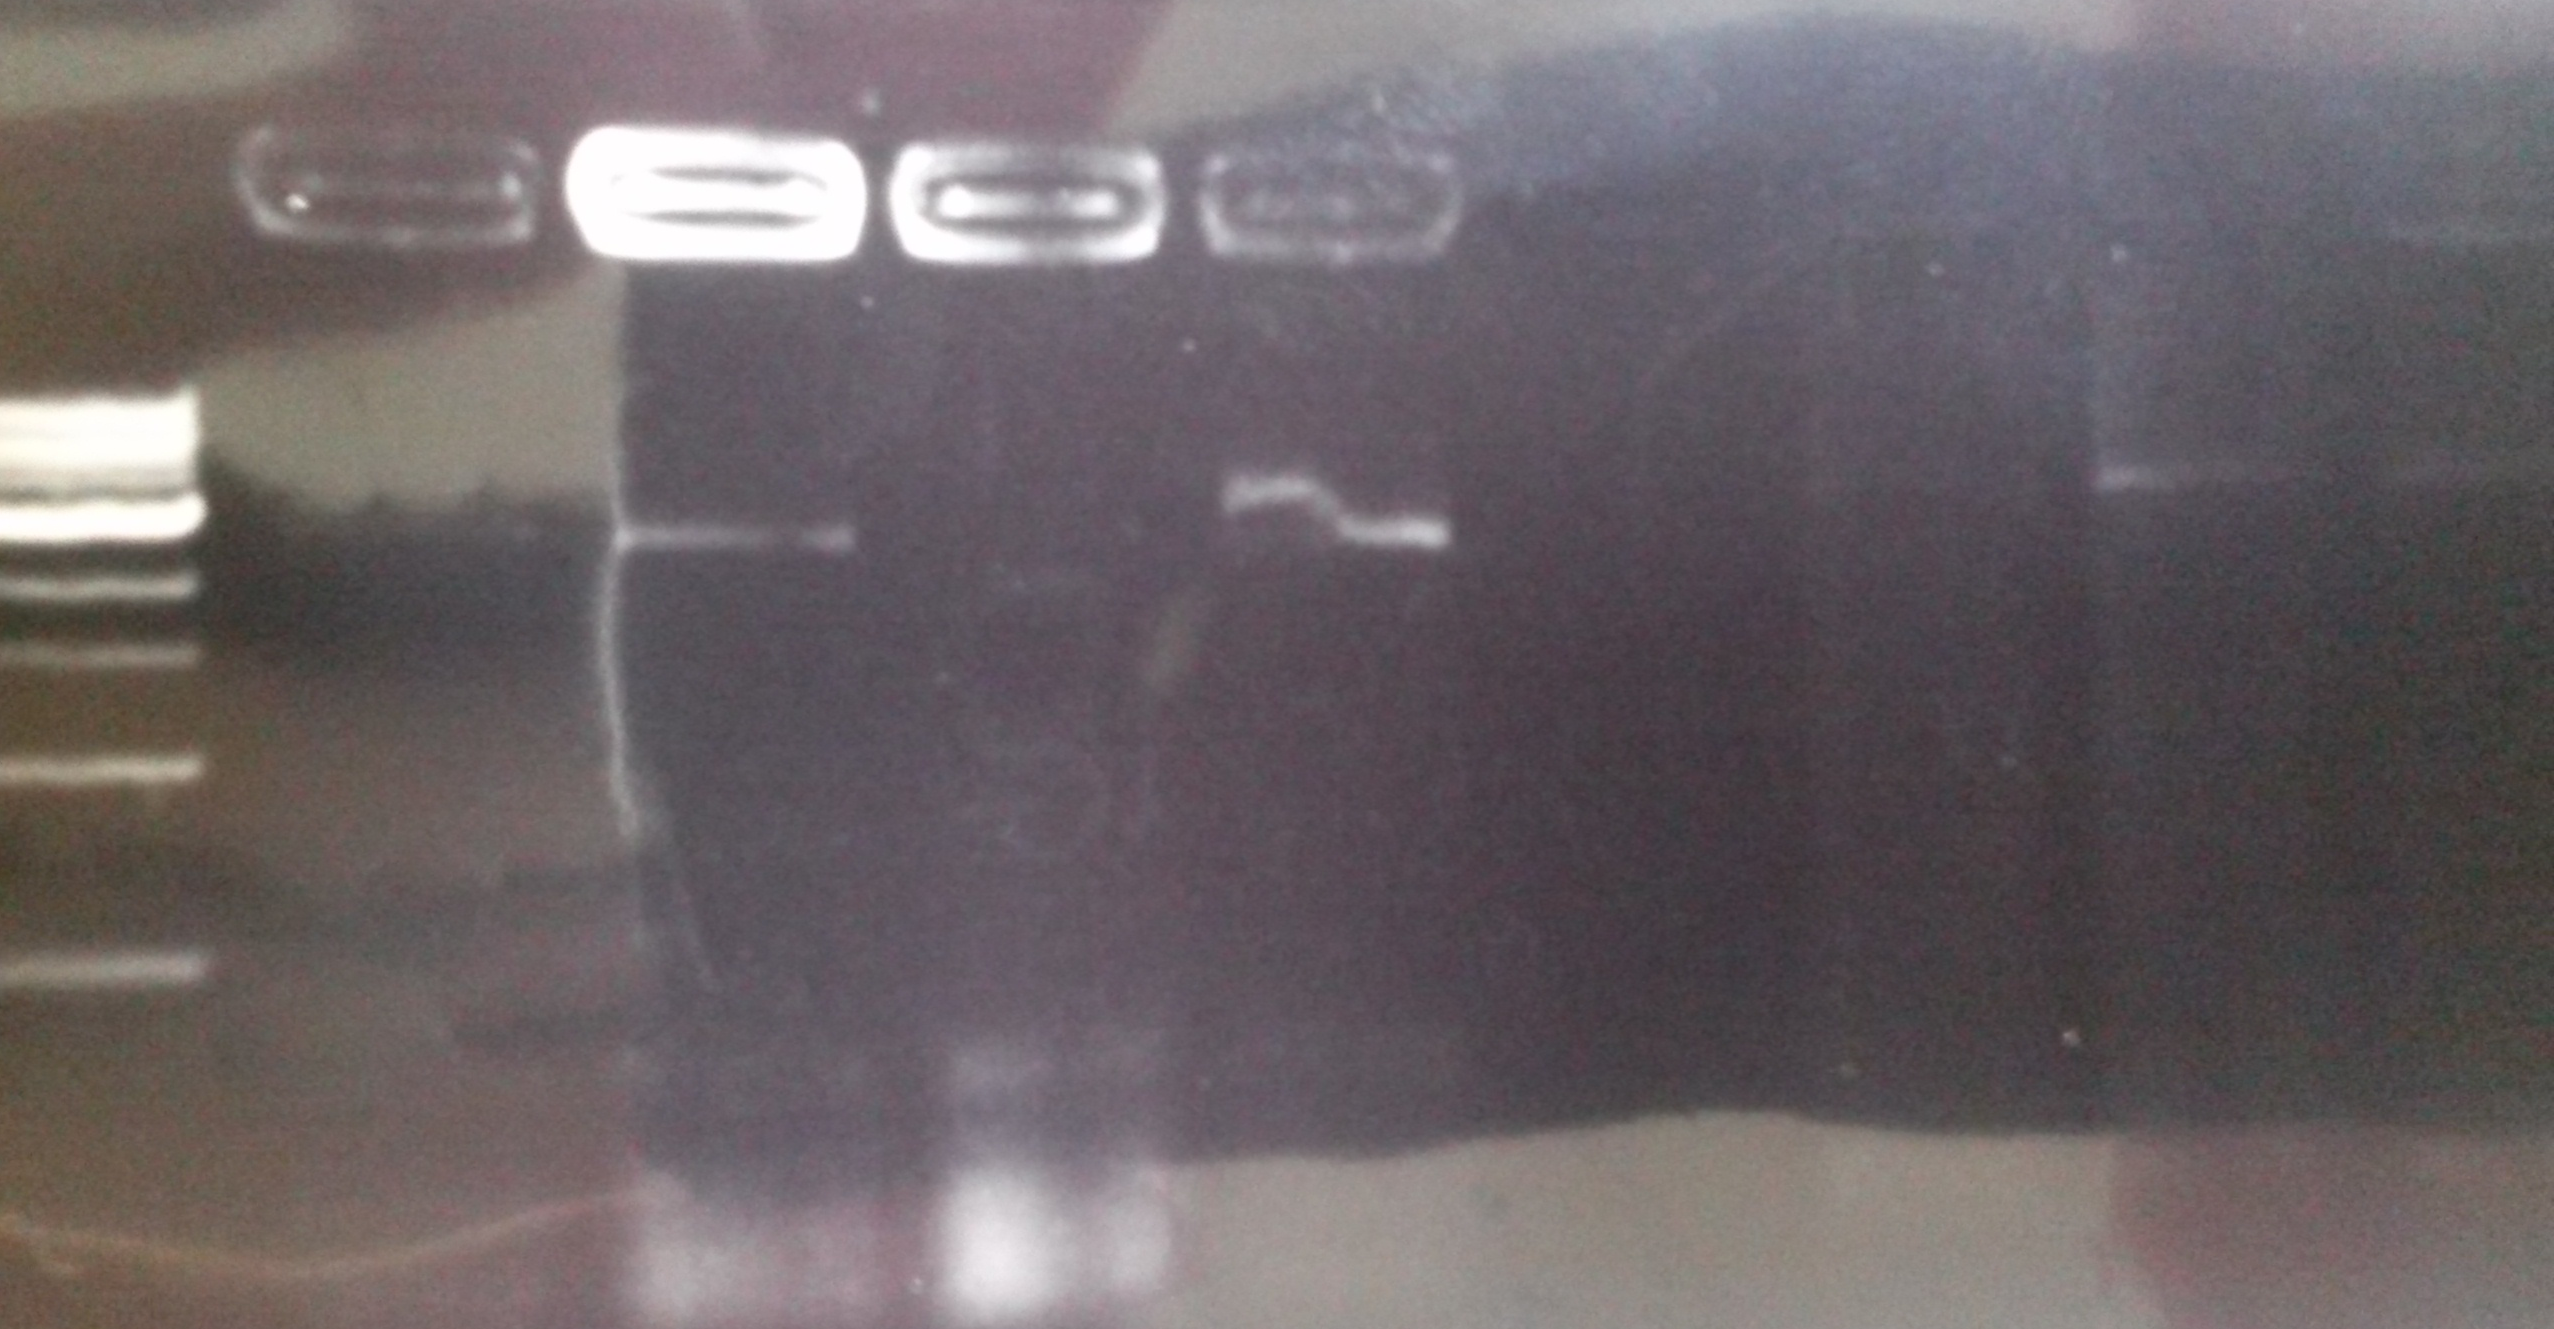
\includegraphics[width=.6\textwidth]{farwtcore1.png}
        \caption{Colony PCR FAR-WT and CORE}
        \label{fig:pcr}
    \end{figure}

    \begin{itemize}
        \item Did a PCR w/ Genomic DNA on 11/14.
    \end{itemize}
\end{frame}


\begin{frame}{Ligation for plasmid creation:}
    \begin{minipage}[ht!]{0.48\textwidth}
        \begin{figure}[ht!]
            \centering
            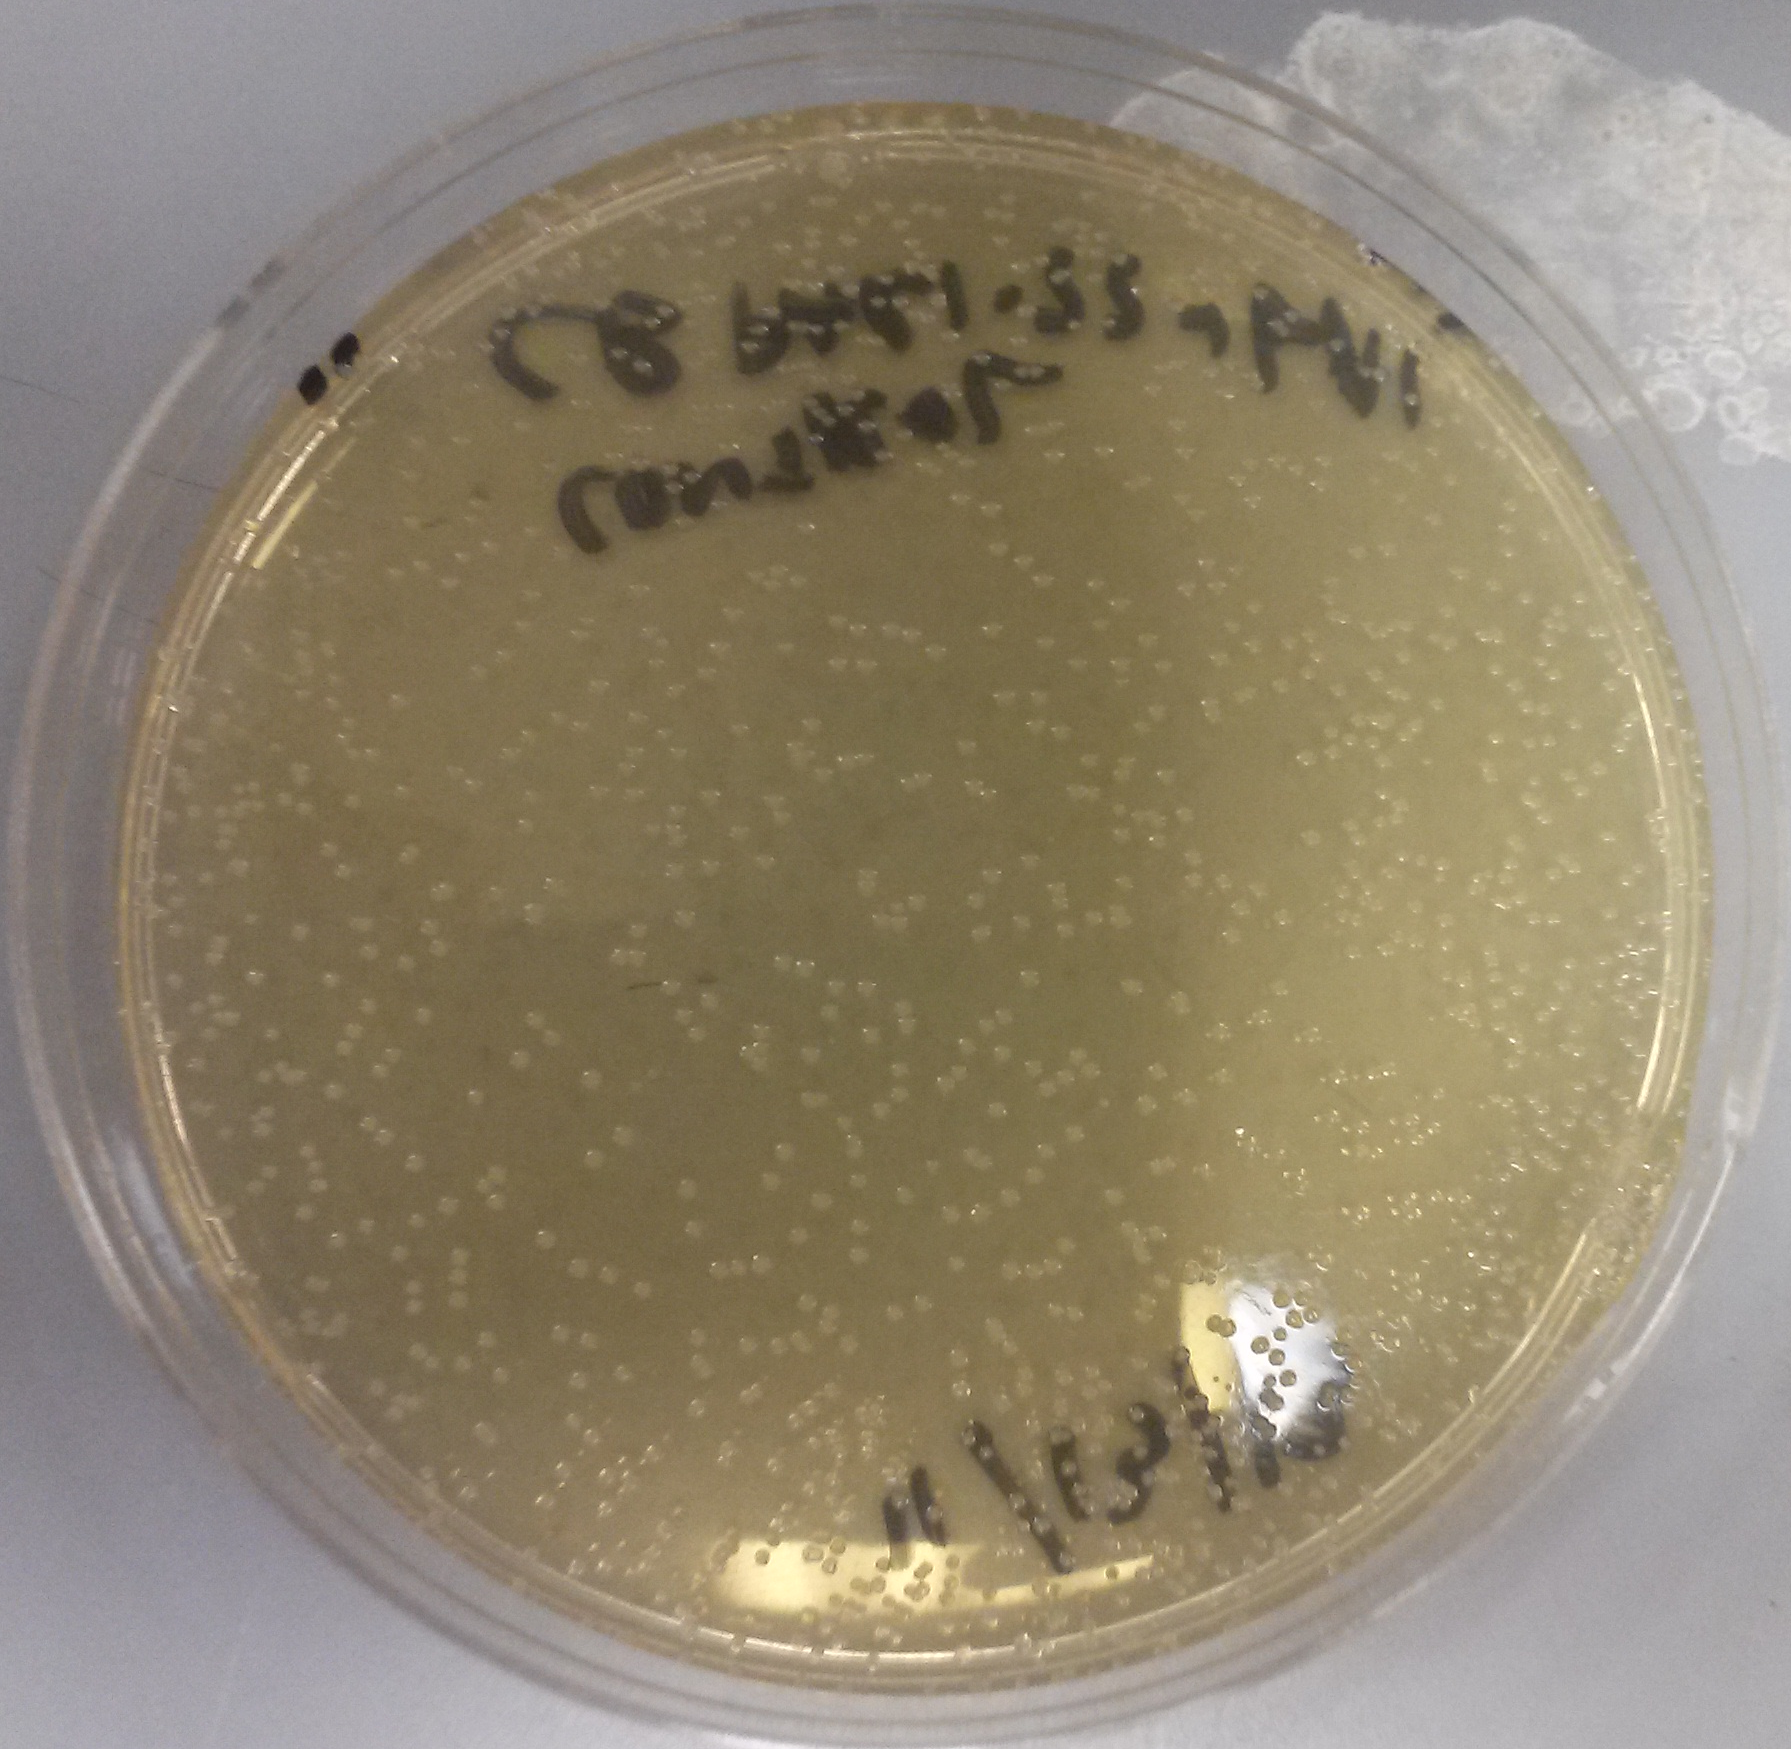
\includegraphics[width=.8\textwidth]{LigControl.png}
            \caption{Ligation Control}
            \label{fig:ligc}
        \end{figure}
    \end{minipage}
    \hfill
    \begin{minipage}[ht!]{0.48\textwidth}
        \begin{figure}[ht!]
            \centering
            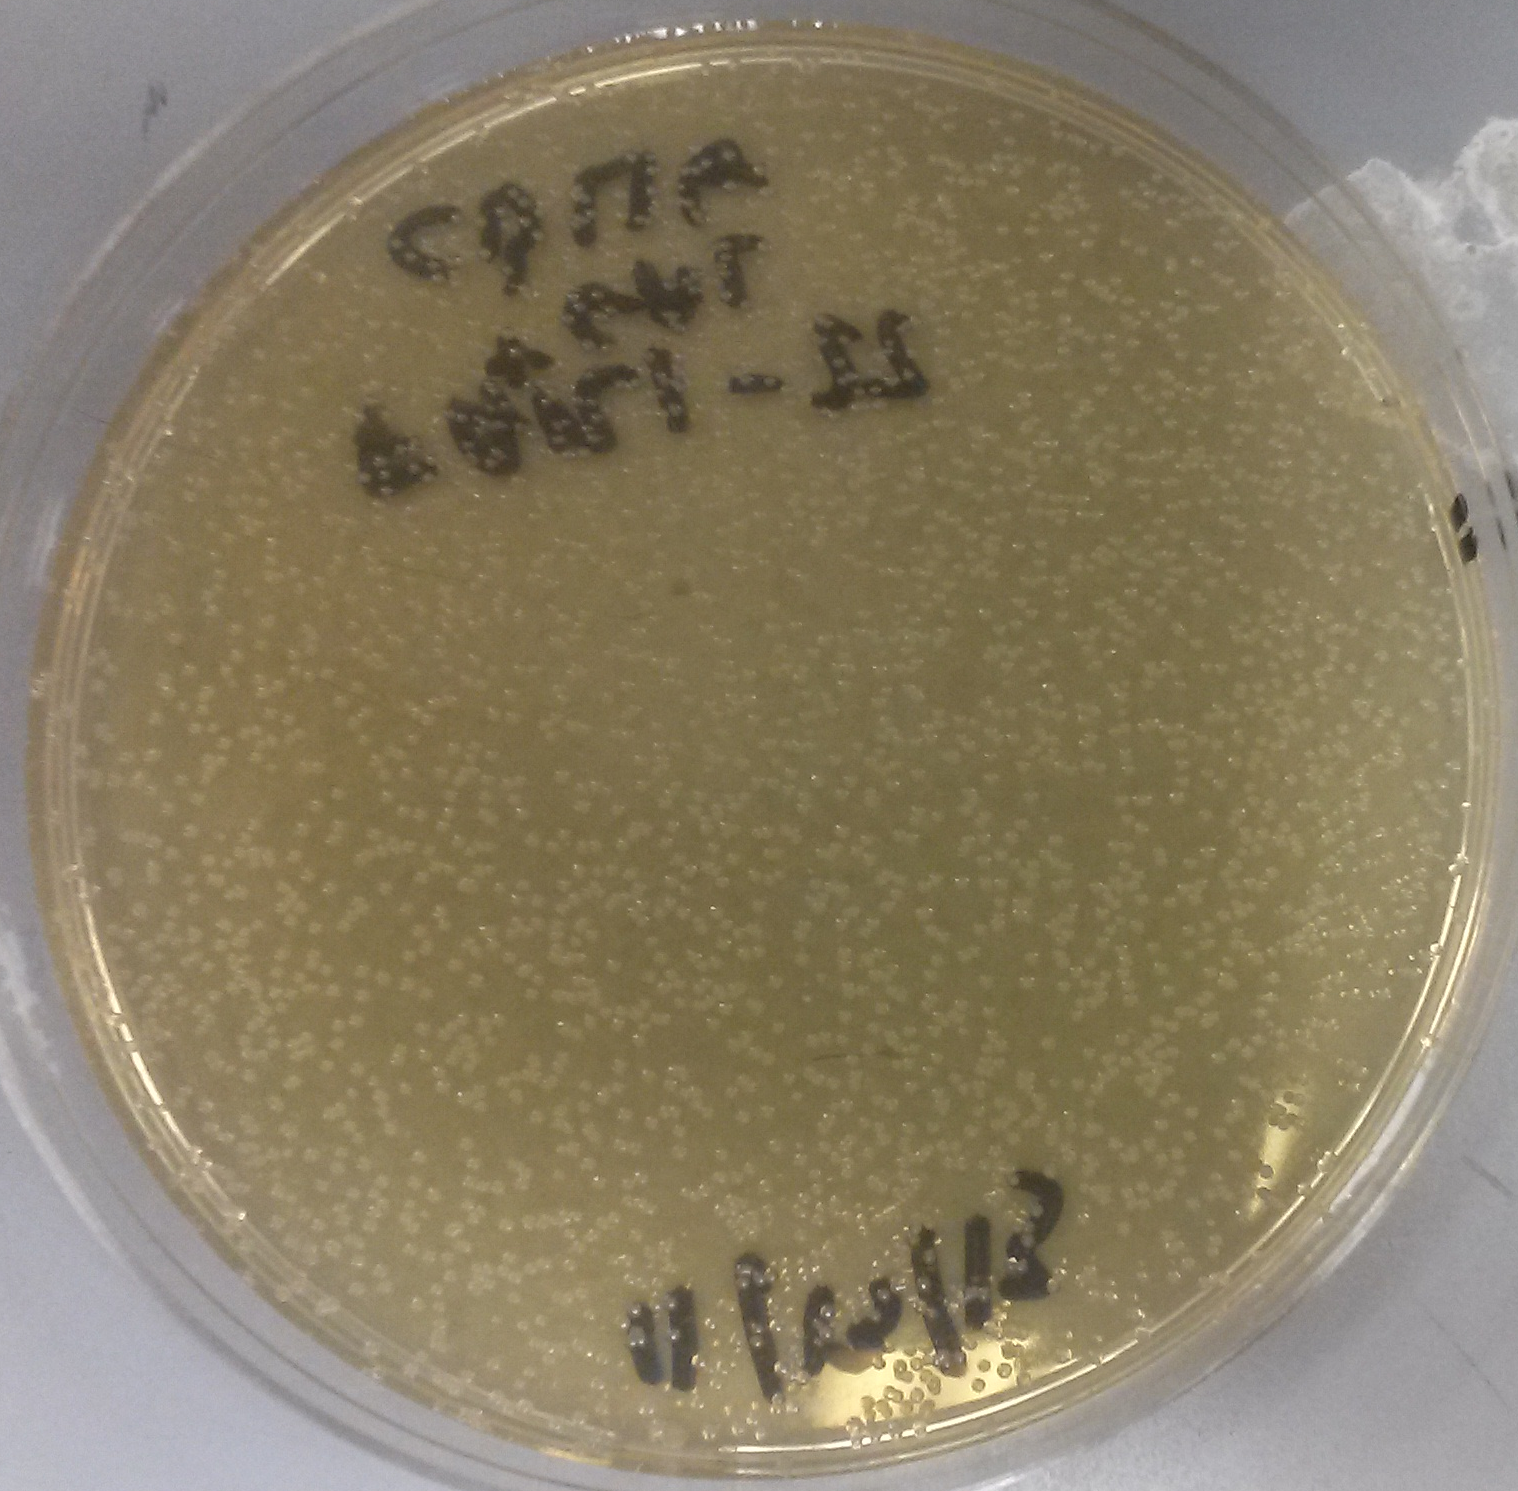
\includegraphics[width=.8\textwidth]{LigVecIns.png}
            \caption{pMM86 with FAR1-22 ligation}
            \label{fig:lig1}
        \end{figure}
    \end{minipage}
\end{frame}


\begin{frame}
    \begin{center}
        {\large \textsc{Steps for Plasmid Construction}}
    \end{center}
        \begin{itemize}
            \item[$\boxtimes$]  Miniprep and digest pMM86
            \item[$\boxtimes$]  Miniprep pGAL-FAR1-22 (pTCN113)
            \item[$\boxtimes$]  PCR amplify FAR1-22 fragment
            \item[$\boxtimes$]  Colony PCR amplify FAR1-WT fragment
            \item[$\boxminus$]  \textbf{Digest both fragments} \textbf{(FAR1-WT)}
            \item[$\boxminus$]  Gel extraction of fragments
            \item[$\boxminus$]  Ligation 
            \item[$\boxminus$] Transformation into bacteria
            \item[$\square$] \textbf{Miniprep and sending to sequencing} (FAR1-22)
            \item[$\square$] Transformation into yeast
        \end{itemize}
\end{frame}


\begin{frame}{Transformation of ZEV with CORE}
    \begin{minipage}[ht!]{0.4\textwidth}
    \begin{figure}[ht!]
        \centering
        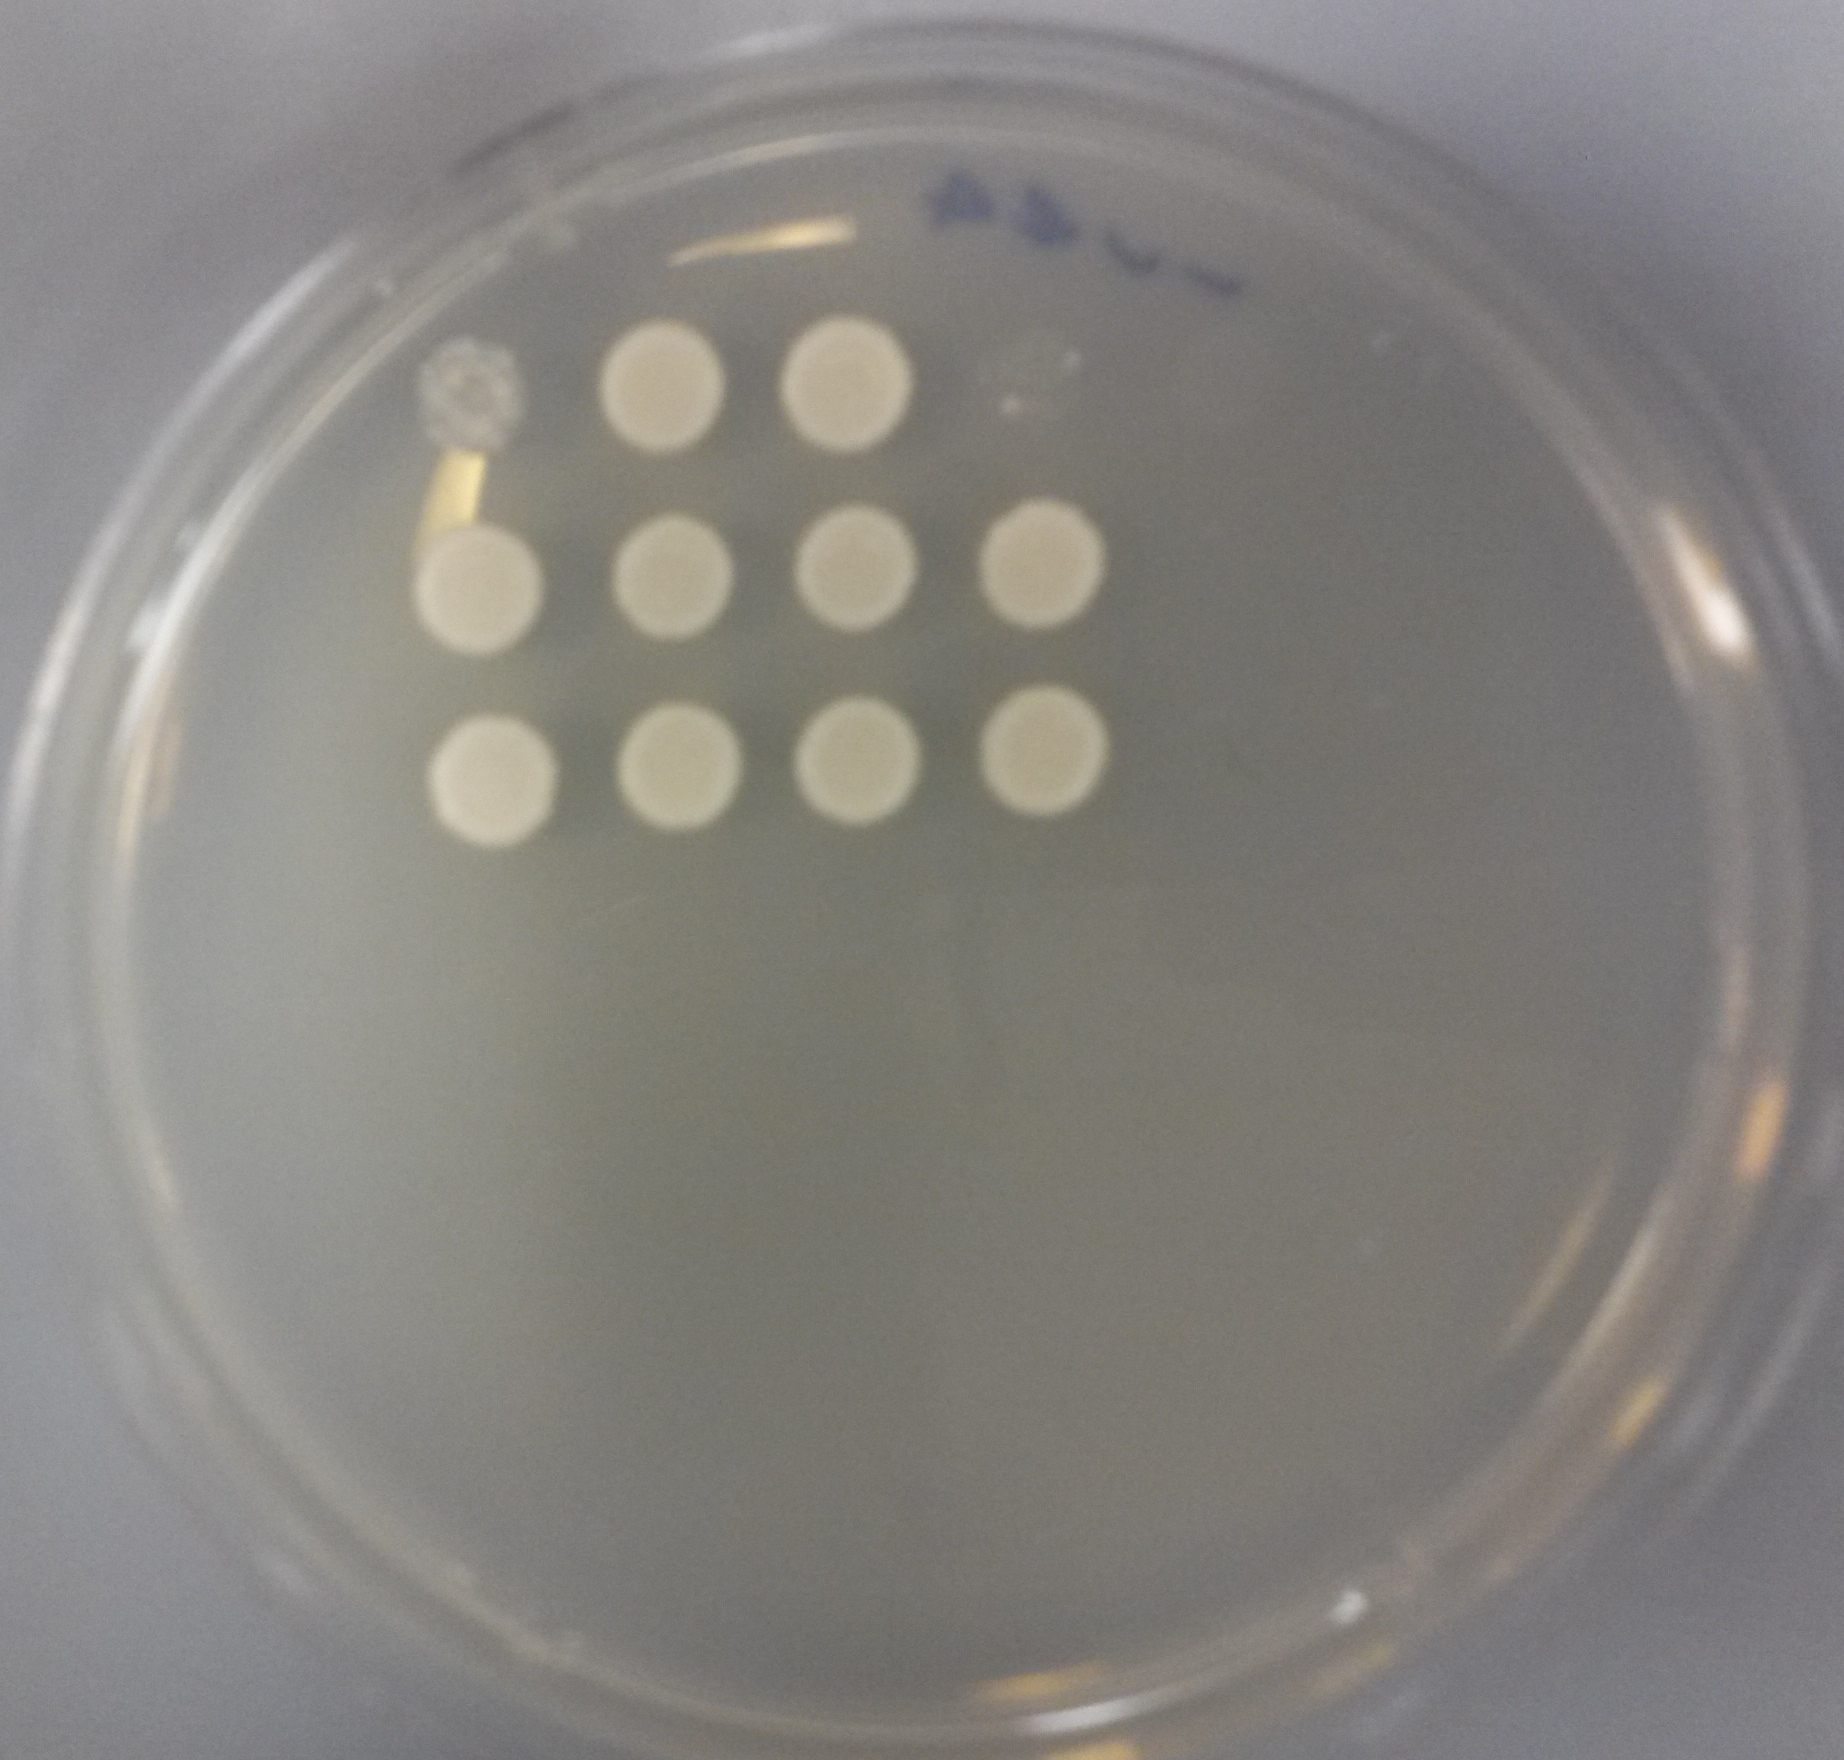
\includegraphics[width=.8\textwidth]{URA.png}
        \caption{URA-}
        \label{fig:ura}
    \end{figure}
    \begin{figure}[ht!]
        \centering
        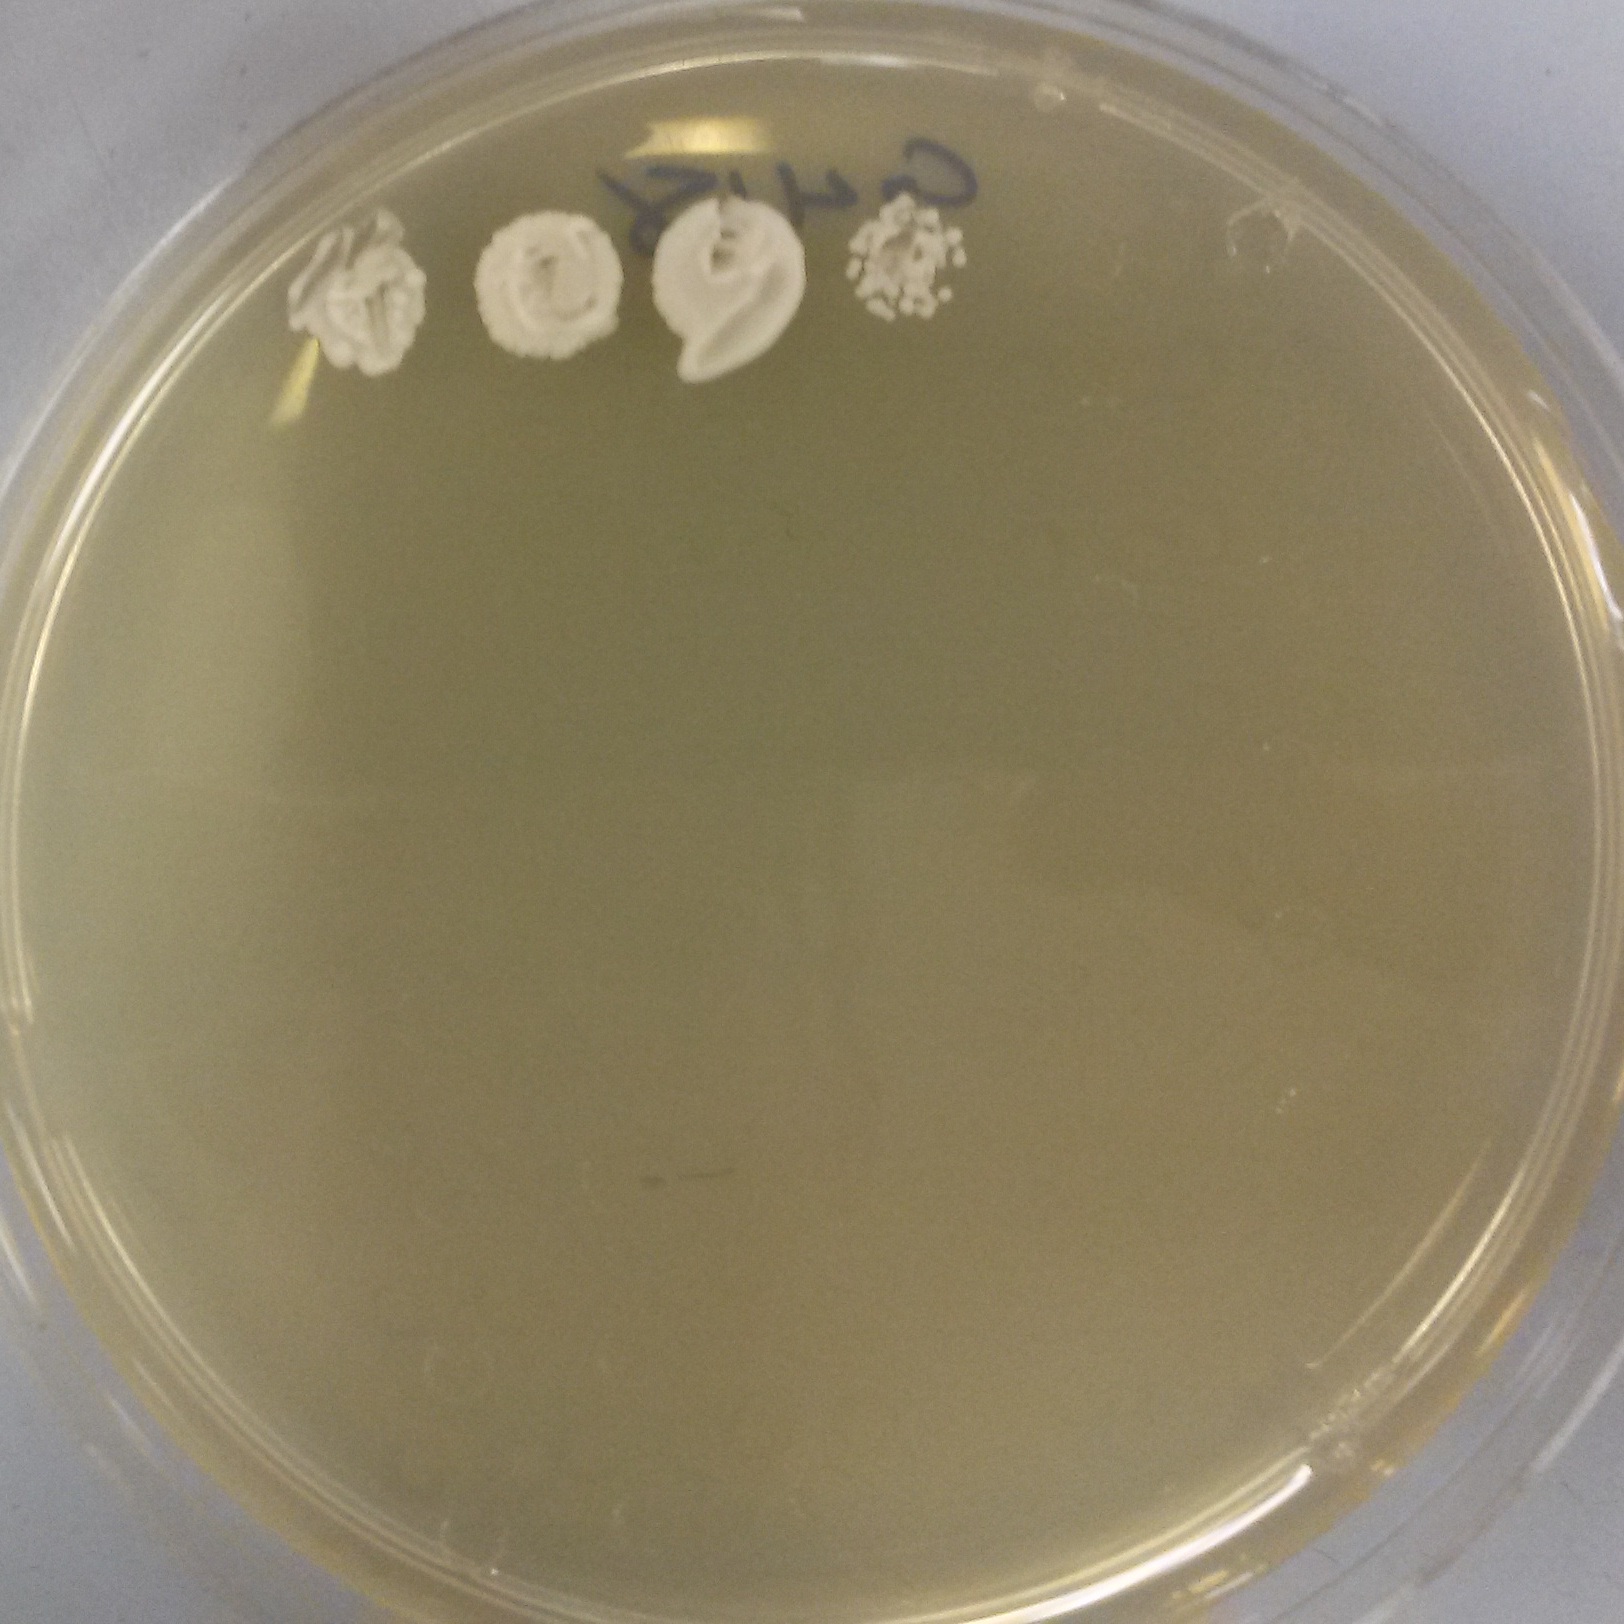
\includegraphics[width=.8\textwidth]{G418.png}
        \caption{G418}
        \label{fig:g418}
    \end{figure}
    \end{minipage}
\hfill
    \begin{minipage}[ht!]{0.4\textwidth}
    \begin{figure}[ht!]
        \centering
        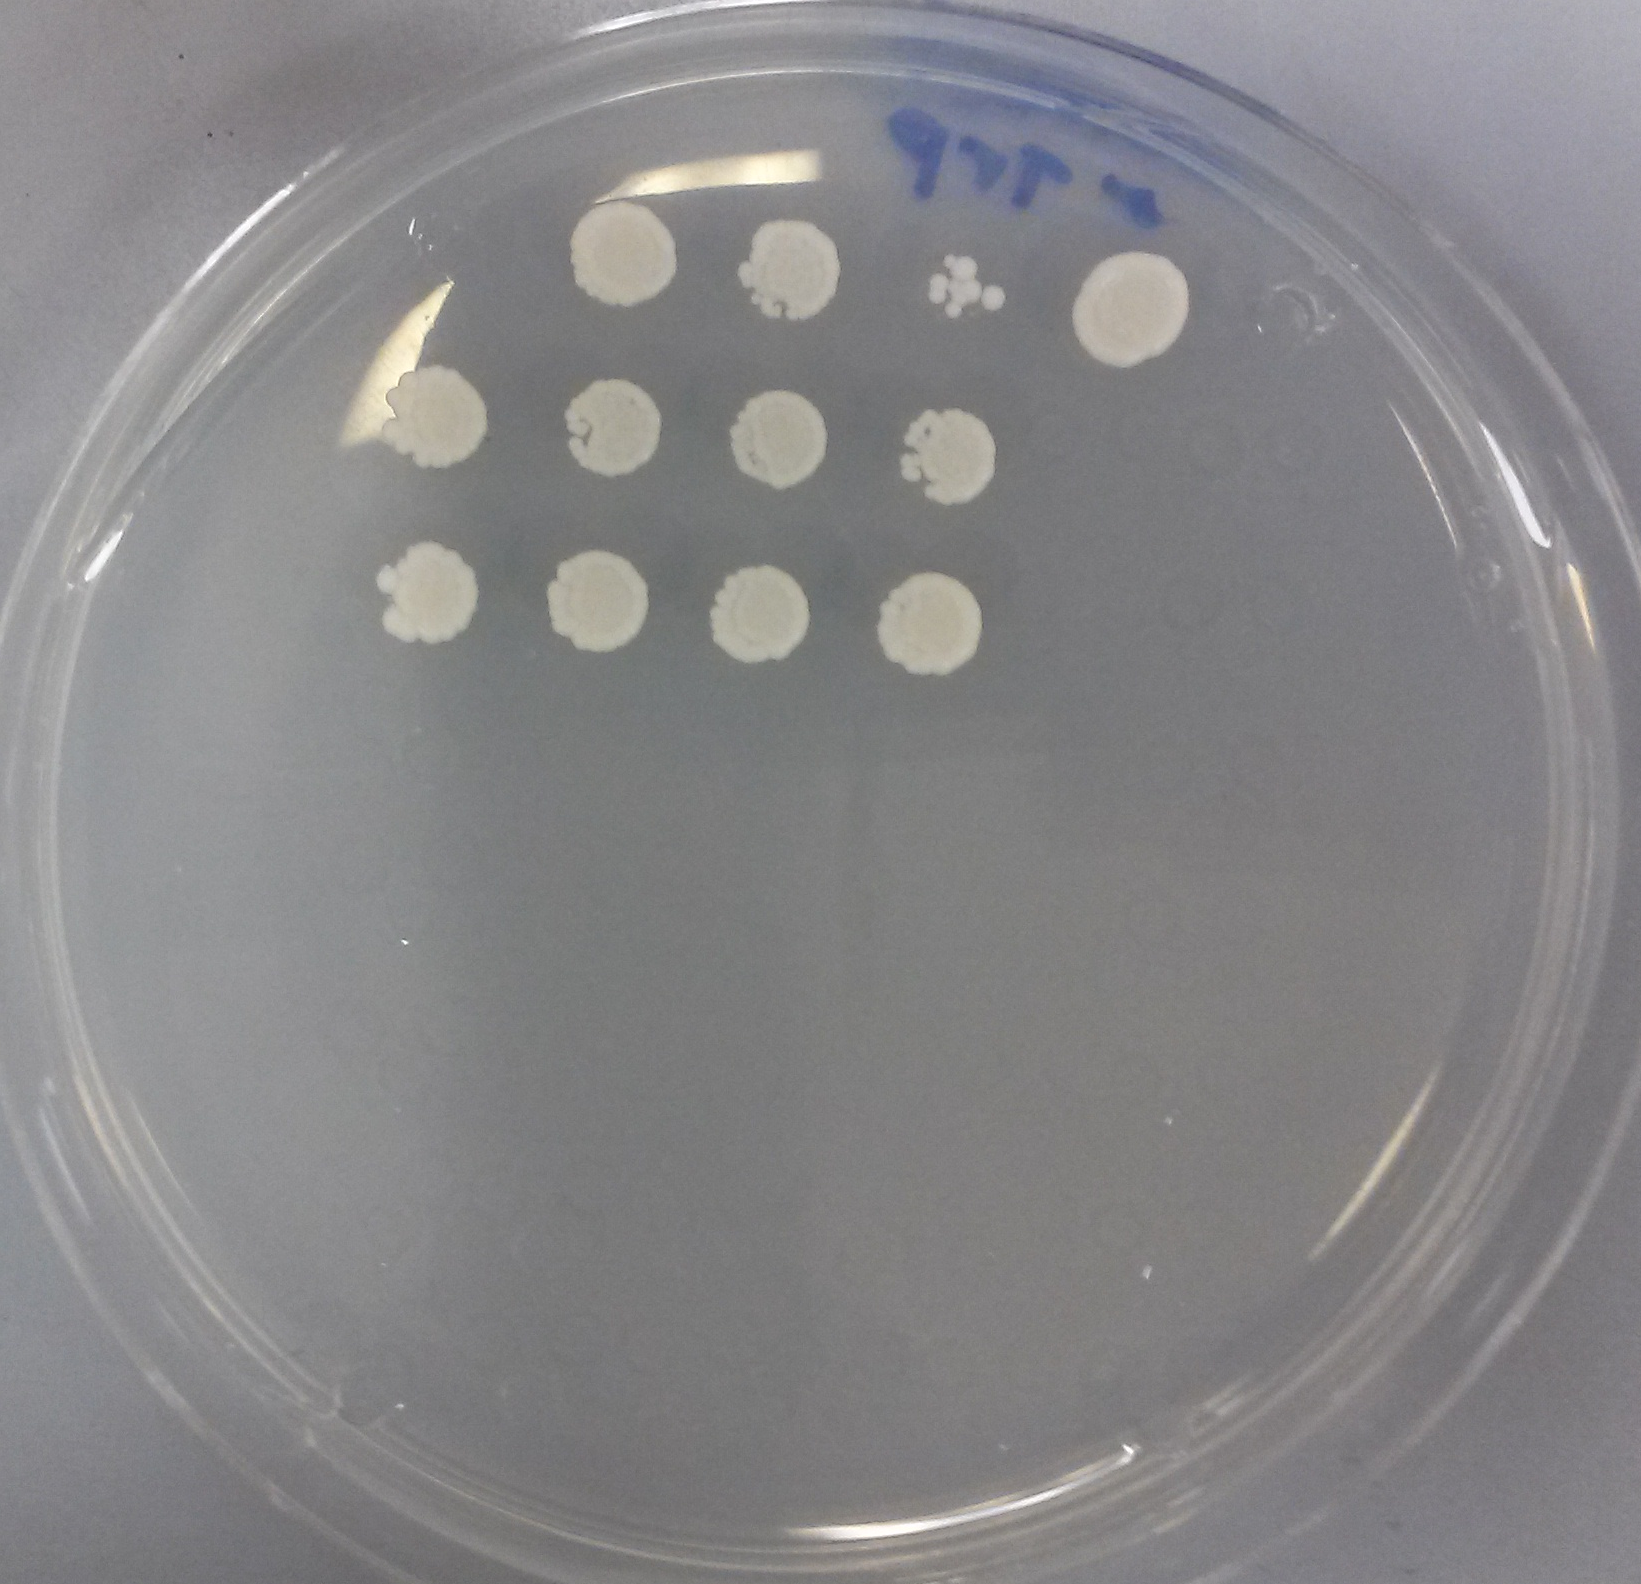
\includegraphics[width=.8\textwidth]{TRP.png}
        \caption{TRP-}
        \label{fig:trp}
    \end{figure}
    \begin{figure}[ht!]
        \centering
        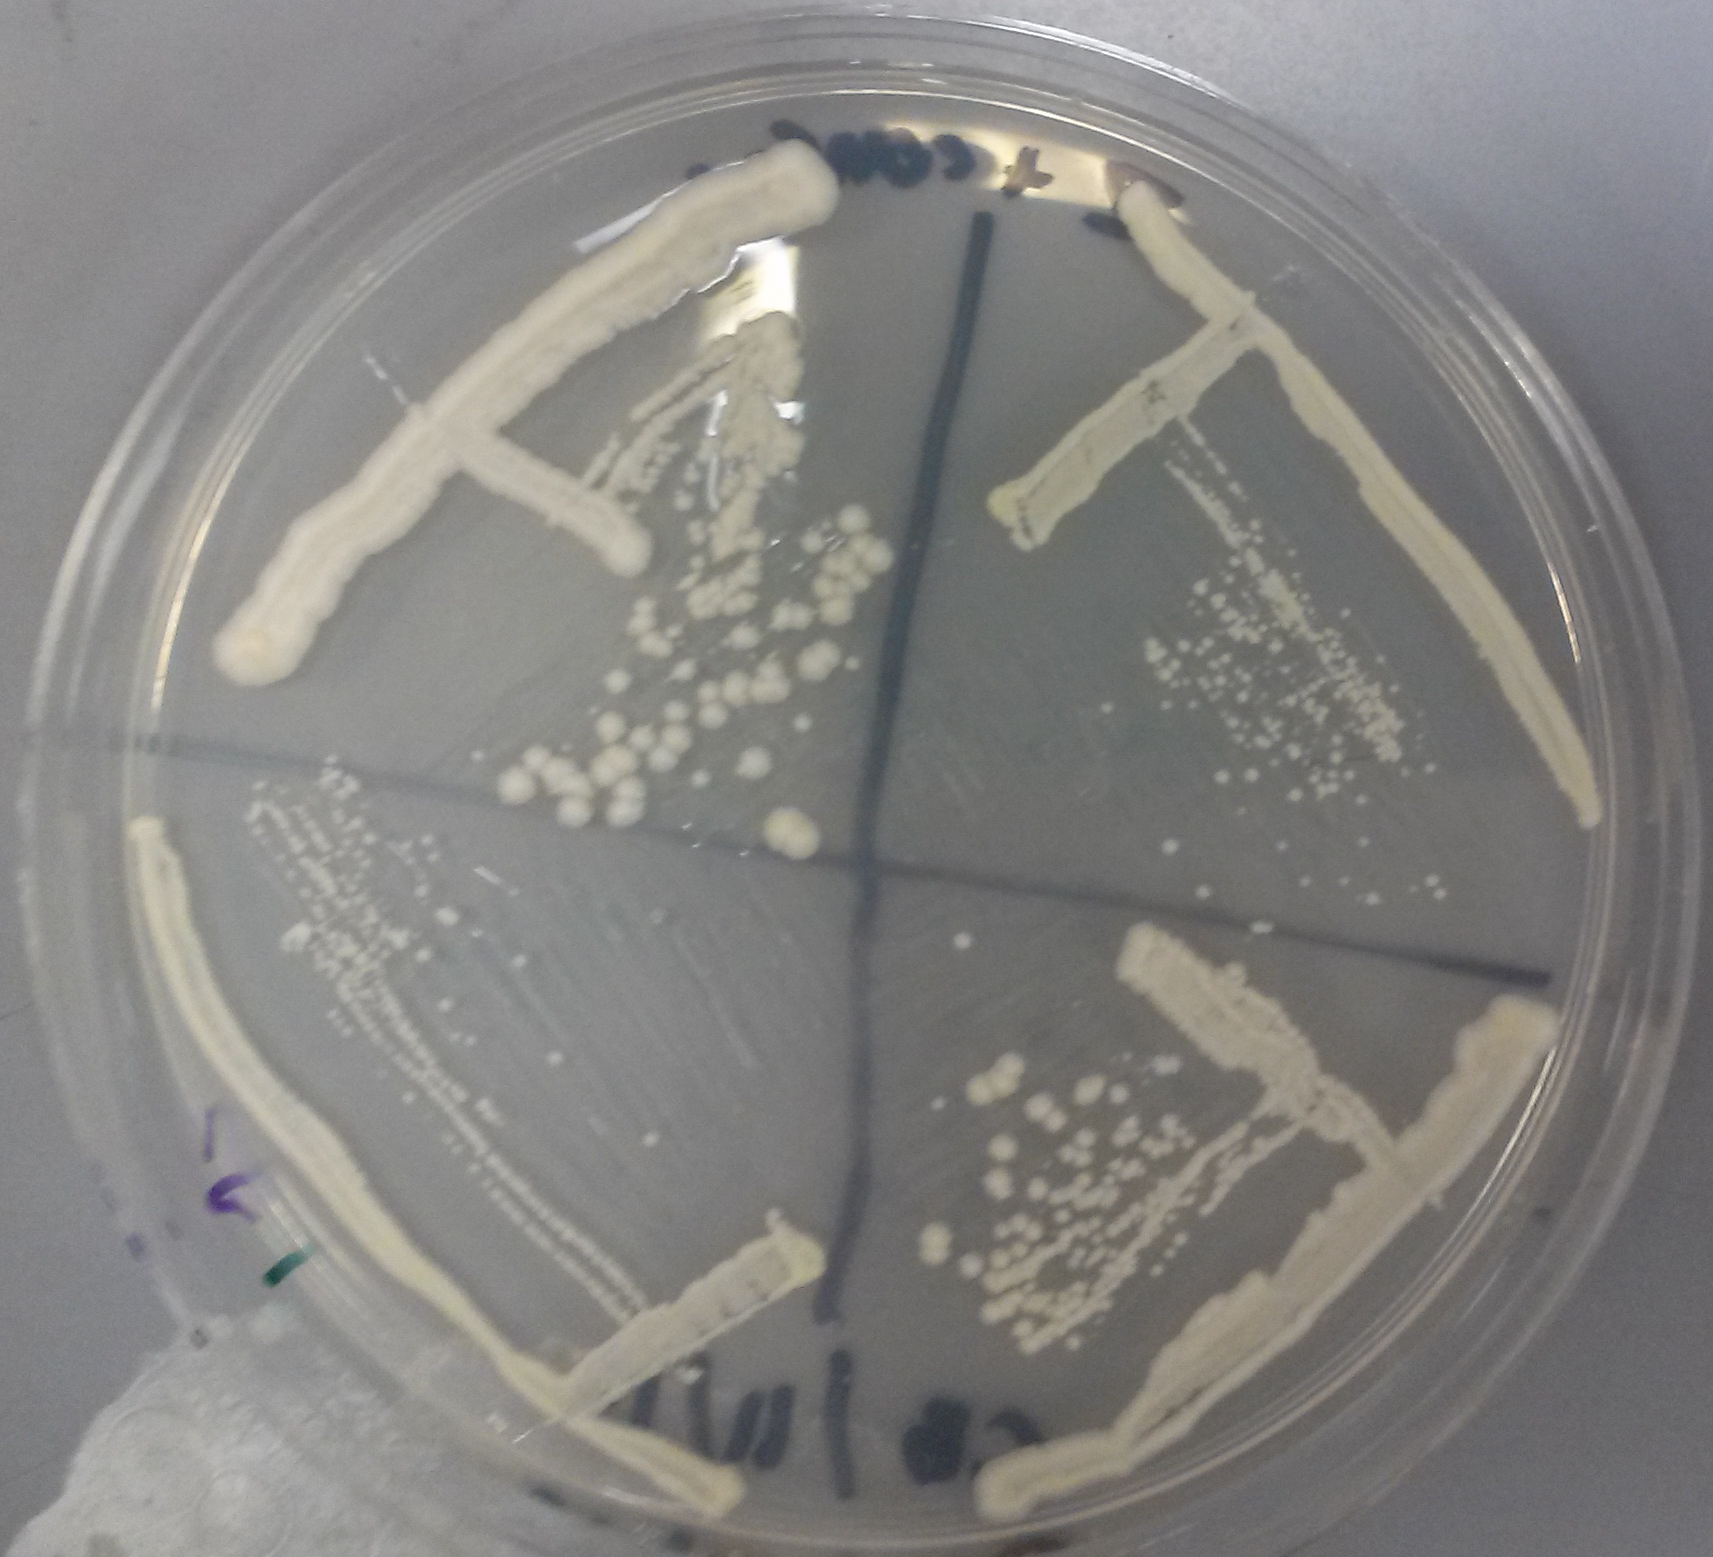
\includegraphics[width=.8\textwidth]{TransformURA2.png}
        \caption{URA-}
        \label{fig:ura2}
    \end{figure}
    \end{minipage}
\end{frame}


\begin{frame}
    \begin{center}
        {\large \textsc{Steps for Genomic Strain Construction}}
    \end{center}
        \begin{itemize}
            \item[$\boxtimes$]  Miniprep pMM299 (ZEVpr)
            \item[$\boxtimes$]  Miniprep pCORE
            \item[$\boxtimes$]  Miniprep pGAL-FAR1-22 (pTCN113)
            \item[$\boxtimes$]  PCR amplify CORE fragment
            \item[$\boxtimes$]  PCR amplify FAR1-22 fragment
            \item[$\boxtimes$]  Colony PCR amplify FAR1-WT fragment
            \item[$\boxtimes$]  Colony PCR amplify ZEVpr fragment
            \item[$\boxtimes$]  Transform ZEV yeast with CORE
            \item[$\square$] \textbf{Transform ZEV+CORE with ZEVpr + FAR fragment}
            \item[$\square$] Send to sequencing.
            \item[$\square$] Transform ZEV + FAR with the blue light plasmids
        \end{itemize}
\end{frame}

\begin{frame}
    \begin{center}
        {\large \textsc{This Week (11/18):}}
    \end{center}

    \textbf{Plasmid Construction:}
    \begin{itemize}
        \item Miniprep of pMM86 + FAR1-22. (pGAL + FAR1-22)\\
        \item Digestion, gel extraction, ligation of FAR1-WT\\
        \item Miniprep + sequencing of FAR1-WT + pMM86.\\
    \end{itemize}
    \textbf{Genomic Construction:}
    \begin{itemize}
        \item Transform ZEV + CORE with FAR1-WT/ FAR1-22 and ZEVpr (homologous recombination).
    \end{itemize}
    \textbf{Controls:}
    \begin{itemize}
        \item Build blue light rig.
        \item Transform ZEV strain with the two blue light plasmids.
    \end{itemize}
    
\end{frame}

% TODO MAKE A PLASMID MAP!!! (OR multiple)


\end{document}
